% !TeX spellcheck = de_AT_frami
\documentclass[10pt,a4paper]{article}
\usepackage[utf8x]{inputenc}
\usepackage{ucs}
\usepackage{amsmath}
\usepackage{setspace}
\usepackage{amsfonts}
\usepackage{amssymb}
\usepackage{graphicx}
\usepackage{txfonts}
\usepackage[dvipsnames]{xcolor}
\usepackage{geometry}
\usepackage{graphicx}
\usepackage{epstopdf}
\epstopdfsetup{update}
\geometry{margin= 2cm}
\usepackage[makeroom]{cancel}
\usepackage{multirow}
\usepackage{mdframed}
\usepackage{listings}
\setlength\parindent{0pt}

\usepackage{scalerel,stackengine}
\stackMath
\newcommand\reallywidehat[1]{%
	\savestack{\tmpbox}{\stretchto{%
			\scaleto{%
				\scalerel*[\widthof{\ensuremath{#1}}]{\kern-.6pt\bigwedge\kern-.6pt}%
				{\rule[-\textheight/2]{1ex}{\textheight}}%WIDTH-LIMITED BIG WEDGE
			}{\textheight}% 
		}{0.5ex}}%
	\stackon[1pt]{#1}{\tmpbox}%
}
\parskip 1ex


\begin{document}
	\pagenumbering{gobble}
	\section*{7. Numerik Übungen 2017/18}
	\paragraph{T12}\mbox{}\\
	\textbf{%
		a) Stellen Sie die Bedingungsgleichung für die Simpsonregel auf und bestimmen Sie damit aus den Knoten $\pmb{c_1=0}$, $\pmb{c_2=\frac{1}{2}}$, und $\pmb{c_3=1}$ die Gewichte.\\
        Welche Ordnung besitzt die Simpsonregel? Untersuchen Sie dazu, ob eventuell noch weitere Bedingungsgleichungen erfüllt sind.
	}\\
	
    
    
    \textbf{%
        b) Gegeben seien die Knoten $\pmb{c_1=\frac{1}{6}}$, $\pmb{c_2=\frac{1}{2}}$, und $\pmb{c_3=\frac{5}{6}}$. Stellen Sie die ersten $\pmb{s}$ Bedingungsgleichungen auf und setzten Sie die Knoten $\pmb{c_1, c_2, c_3}$ ein. Berechnen Sie daraus die Gewichte. Wie groß ist die Ordnung dieser Quadraturformel?
    }\\


    \textbf{%
        c) Bestimmen Sie alternativ die Gewichte $\pmb{b_1, b_2, b_3}$ durch Integration der zu den Knoten $\pmb{c_1, c_2, c_3}$ gehörigen Lagrange-Polynome $\pmb{l_1, l_2, l_3}$.
    }\\


    \textbf{%
        d) Welche Ordnung hat eine Quadraturformel mit Knoten wie in (T12b) und Gewichten $\pmb{b_1=\frac{1}{3}, b_2=\frac{1}{3}, b_3=\frac{1}{3}}$?
    }\\



    \pagebreak
    \paragraph{T13}\mbox{}\\
    \textbf{%
        Berechnen Sie das Integral
        \begin{align*}
            \pmb{\int_{-1}^{2}\frac{1}{2+x}dx}.
        \end{align*}
        a) Exakt.}\\
        Substitution mit $\xi=2+x$ und $du=d\xi$.
        \begin{align*}
            \int_{u}^{o}\frac{1}{\xi}d\xi = \text{log}(\xi)\arrowvert^o_u = \text{log}(x+2)\arrowvert^2_{-1} = \text{log}(4)-\text{log}(1) = \text{log}\left(\frac{4}{1}\right)=\text{log}(4)\approx1.3863
        \end{align*}
        
        \textbf{%
        b) Mit der Quadraturformel aus Aufgabe (T12b) und Schrittweite $\pmb{h=3}$.
        }\\
	    Auszug Definition 4.2 (S. 80):
	    \begin{mdframed}[linewidth=0pt,backgroundcolor=gray!20]
	    Für eine äquidistante Unterteilung von [a, b] in $n$ Teilintervalle, also
	    \begin{align}\tag{4.22}
		    x_k = a + k h,\quad h = \frac{b-a}{n} ,\quad k=0,\dots,n
	    \end{align}
	    haben wir folgende Näherungsformel:
		\begin{align}\tag{4.23}
			\int_{a}^{b}f(x)dx \approx h\sum_{k=1}^{n}\sum_{i=1}^{s}b_if(x_{k-1}+c_ih)
		\end{align}
	\end{mdframed}
	    \begin{align*}
		    h=3=\frac{2+1}{n} &\Rightarrow n=1, \quad x_0=a=-1 ,\quad s=3, \quad
		    c = \begin{bmatrix}
			    \frac{1}{6} \\
			    \frac{1}{2} \\
			    \frac{5}{6}
		    \end{bmatrix}, \quad  b= \begin{bmatrix}
		    	\frac{3}{10} \\
		    	\frac{2}{5}  \\
		    	\frac{3}{10}
		    \end{bmatrix} \\
		\int_{-1}^{2}\frac{1}{2+x}dx &\approx 3\sum_{k=1}^{1}\sum_{i=1}^{3}b_if(x_{1-1}+c_i\cdot3) \\
	    &\approx 3\sum_{i=1}^{3}b_if(x_{0}+3c_i) \\
	    &\approx 3\left[b_1f(x_{0}+3c_1)+b_2f(x_{0}+3c_2)+b_3f(x_{0}+3c_3) \right] \\
	    &\approx 3\left[b_1f(-1+3\frac{1}{6})+b_2f(-1+3\frac{1}{2})+b_3f(-1+3\frac{5}{6})\right]  \\
	    &\approx 3\left[\frac{3}{10}f(-\frac{1}{2})+\frac{2}{5}f(\frac{1}{2})+\frac{3}{10}f(\frac{3}{2})\right]  \\
	    &\approx 3\left[\frac{3}{10}\frac{2}{3}+\frac{2}{5}\frac{2}{5}+\frac{3}{10}\frac{2}{7}\right]  \\
	    &\approx 1.337142857142857 \quad (96.45\%)
	    \end{align*}
	    
	    \newpage
        \textbf{%
        c) Mit der Quadraturformel aus Aufgabe (T12b) und Schrittweite $\pmb{h=\frac{3}{2}}$. \\
        Machen Sie eine Skizze mit den Knoten und Gewichten.
		}\\
        \begin{align*}
        h=\frac{3}{2}=\frac{2+1}{n} &\Rightarrow n=2, \quad x = \begin{bmatrix}
	        -1\\ \frac{1}{2}
        \end{bmatrix} ,\quad s=3, \quad
        c = \begin{bmatrix}
        \frac{1}{6} \\
        \frac{1}{2} \\
        \frac{5}{6}
        \end{bmatrix}, \quad  b= \begin{bmatrix}
        \frac{3}{10} \\
        \frac{2}{5}  \\
        \frac{3}{10}
        \end{bmatrix} \\
        \int_{-1}^{2}\frac{1}{2+x}dx &\approx \frac{3}{2}\sum_{k=1}^{2}\sum_{i=1}^{3}b_if(x_{k-1}+c_i\cdot\frac{3}{2}) \\
        &\approx \frac{3}{2}\left[\left(  b_1f(x_0+\frac{3}{2}c_1)+b_2f(x_0+\frac{3}{2}c_2)+b_3f(x_0+\frac{3}{2}c_3)\right)+\left(
        b_1f(x_1+\frac{3}{2}c_1)+b_2f(x_1+\frac{3}{2}c_2)+b_3f(x_1+\frac{3}{2}c_3) \right)  \right] \\
        &\approx \frac{3}{2}\left[\left(  \frac{3}{10}f(-1+\frac{3}{2}\frac{1}{6})+\frac{2}{5}f(-1+\frac{3}{2}\frac{1}{2})+\frac{3}{10}f(-1+\frac{3}{2}\frac{5}{6})\right)+\left(
        \frac{3}{10}f(\frac{1}{2}+\frac{3}{2}\frac{1}{6})+\frac{2}{5}f(\frac{1}{2}+\frac{3}{2}\frac{1}{2})+\frac{3}{10}f(\frac{1}{2}+\frac{3}{2}\frac{5}{6}) \right)  \right] \\
        &\approx \frac{3}{2}\frac{1}{5}\left[\left(  \frac{3}{2}f(-\frac{3}{4})+2f(-\frac{1}{4})+\frac{3}{2}f(\frac{1}{4})\right)+\left(
        \frac{3}{2}f(\frac{3}{4})+2f(\frac{5}{4})+\frac{3}{2}f(\frac{7}{4}) \right)  \right] \\
        &\approx \frac{3}{10}\left[\left(  \frac{3}{2}\frac{4}{5}+2\frac{4}{7}+\frac{3}{2}\frac{4}{9}\right)+\left(
        \frac{3}{2}\frac{4}{11}+2\frac{4}{13}+\frac{3}{2}\frac{4}{15} \right)  \right] \\
        &\approx \frac{3}{10}\left[\left(  \frac{12}{10}+\frac{8}{7}+\frac{2}{3}\right)+\left(
        \frac{6}{11}+\frac{8}{13}+\frac{6}{15} \right)  \right] \\
        &\approx 1.3711088911088911 \quad (98.90\%)
       \end{align*}
       \begin{figure}[htbp]
	       	\centering
	       	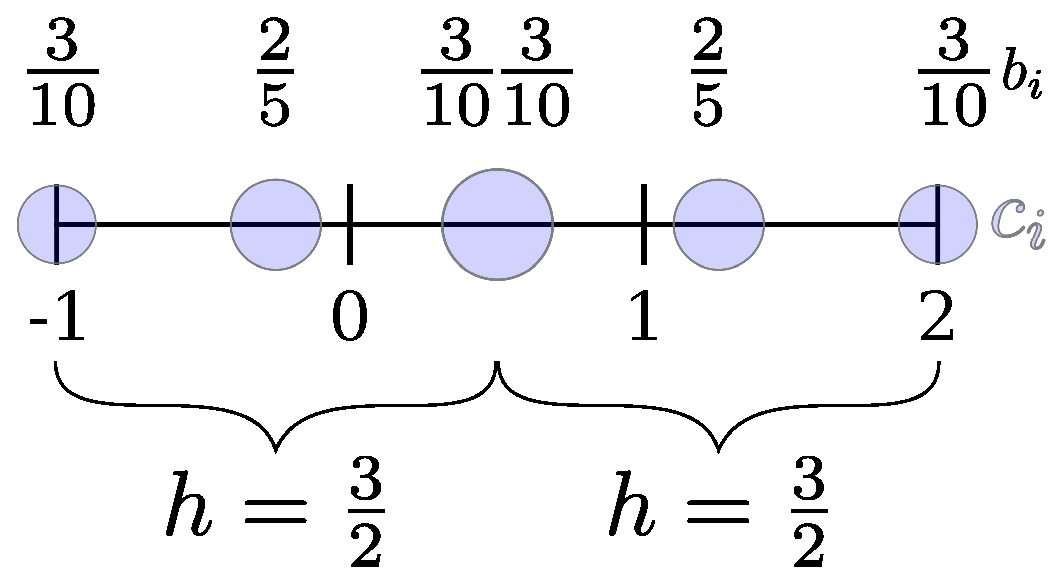
\includegraphics[scale=0.3]{T13}
       \end{figure}\\ 
       Python 3.5
       \begin{mdframed}[linewidth=0pt,backgroundcolor=gray!10]
	   \lstinputlisting[language=Python]{T13c.py}
	\end{mdframed}
\end{document}